\scanpage{72}
% archive sheet number: 71

$\underline{Q}_p$ faisceaux constructibles sur $k$ vers la catégorie $\mathrm{Fcriso}(k)$. Pour un objet \deleted{\unsure{$E$}}$(E,F_E)$ de cette dernière, les conditions suivantes sont équivalentes\inserted{(si $k$ parfait)}: a) $(E,F_E)$ appartient à l'image essentielle du foncteur précédent; b) il existe un réseau $M\subset E$ stable par $F_E$ \deleted{\unsure{sur}} \uline{et} par $F_E^{-1}$ (i.e. tel que $F_E$ induise un \uline{automorphisme} de $M$); c) la famille des i\handwritten{t}érés $F^{\unsure{m|n}}$, $n\quad\underline{Z}$, est bornée ; d) $E$ et $E^{\handwritten{\vee}}$ sont effectifs.

Les F-isocristaux en question sont appelés ``trivaux'' ou ``\uline{de pente nulle}''. On trouve ainsi un \uline{épimorphisme de gerbes}
\figure{\[
\underline{G}(k)\handwritten{\longrightarrow}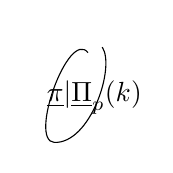
\begin{tikzpicture}[baseline=(gerbe.base)]
\node[inner sep=1pt] (gerbe) {$\handwritten{\unsure{\underline{\pi}|\underline{\Pi}}_{p}}(k)$};
\handwritten{\draw[thin] (-0.08,0.57) .. controls (-0.33,0.88) and (-0.84,-0.55) .. (-0.51,-0.57) .. controls (-0.05,-0.59) and (0.27,0.39) .. (0.10,0.64);}
\end{tikzpicture}\ ,
\]}
\margin{\handwritten{$\Pi$\par majuscule?}}
où $\handwritten{\underline{\pi}}_p(k)$ est la gerbe sur $\underline{Q}_p$ \deleted{des représentations continues} associée à la catégorie tannakienne des $\underline{Q}_p$-faisceaux constructibles, équivalente \deleted{à l'enveloppe alg} (une fois choisie une clôture algébrique $\bar{k}$ de $k$) à la gerbe triviale définie par l'enveloppe algébrique \deleted{du} $p$-adique du groupe pro-fini $\handwritten{\pi}=\operatorname{Gal}(\handwritten{\bar{k}}/k)$. Tenant compte de l'homomorphisme d'augmentation de \unsure{Gate|Tate}, on trouve même un homomorphisme
\[
\underline{G}(k)\handwritten{\longrightarrow\underline{\pi}}_p(k)\ \mathrm{x}\ \handwritten{[}\underline{G}_m\handwritten{]}_{\underline{Q}_p}
\]
où $\handwritten{[}\underline{G}_m\handwritten{]}$ est la gerbe triviale définie par $\underline{G}_m$ . On vérifie facilement que c'est encore un épimorphisme (i.e. que le foncteur
\[
(V_i)_{\handwritten{i}}\handwritten{\longmapsto\sum}V_i\otimes_{\underline{\mathbb{Q}}_p}\underline{Q}_p(i)
\]
allant de la catégorie des \deleted{\unsure{sh}} $\underline{Q}_p$-faisceaux constructibles \inserted{\handwritten{gradués}} sur $k$ vers $\mathrm{Fcriso}(k)$ est pleinement fidèle). Les F-isocristaux de la forme précédente pourraient être appelés les F-isocristaux \uline{de niveau zéro} .

\handwritten{6.} Considérons maintenant un \unsure{homomorphisme} de corps\deleted{x}
\[
k\handwritten{\longrightarrow}k'\ ,
\]
d'où un homomorphisme de catégories tannakiennes sur $\underline{Q}_p$
\[
\mathrm{Fcriso}(k)\handwritten{\longrightarrow}\mathrm{Fcriso}(\handwritten{k}')\ ,
\]
et un homomorphisme de gerbes tannakiennes sur $\underline{Q}_p$ en sens inverse
